\documentclass[conference]{IEEEtran}
\usepackage{graphicx,booktabs,url}
\title{ForgeryLens: Can a Single Receipt Image Prioritize Manual Review?}
\author{\IEEEauthorblockN{Mohsin Saeed, Hamza Sami, and M. Taha}\IEEEauthorblockA{Ghulam Ishaq Khan Institute of Engineering Sciences and Technology, Pakistan\\AI341 Deep Neural Networks}}
\begin{document}
\maketitle
\begin{abstract}
A university finance office needs to find edited receipts early while keeping manual review manageable. We evaluated a native-patch MobileNetV3-Small on original and edited receipt images, grouping possible aliases before fitting on 556 source groups. On historical WildReceipt, the model achieved AUROC 0.5015 and expected calibration error 0.0106. The frozen review policy prioritized zero of 1,336 edits, routed six edited receipts to the normal queue, and deferred 2,660 of 2,672 documents. The model used 927,585 parameters and required 156 ms median on a laptop CPU. Interventions on matched receipts showed that an edit could change its local tile score without changing the document decision. These results support manual review and identify where evidence is lost.
\end{abstract}
\begin{IEEEkeywords}
receipt forensics, distribution shift, selective classification, document review
\end{IEEEkeywords}
\section{Decision and requirements}
A priority flag moves a reimbursement claim earlier in a finance reviewer's queue. A normal-queue outcome retains the standard checklist. An inconclusive outcome returns the claim to manual review. Staff verify transaction records and authorized revisions before deciding on payment. A visual change alone cannot establish fraud.

The finance reviewer prioritizes edited-receipt recall of at least 90\%, counting deferred edits as missed priority opportunities. The claimant needs protection against unnecessary escalation: proposed budgets are at most 5\% genuine false flags and 100 priority reviews per 1,000 receipts. Third in priority, audit staff require shifted macro F1 of at least 0.75. Fourth, confidence should support ten-bin ECE at most 0.10, coverage at least 50\%, and accepted error at most 10\%. Fifth and sixth, IT requires batch-one median latency at most 100 ms and at most 25M parameters. We report p95 to expose the cost of large receipts.

Lowering the review cutoff can overload reviewers; increasing the confidence threshold transfers work to the manual queue. Actual prevalence and staffing capacity are unknown. At an illustrative 1\% edit prevalence, the observed development rates of 12.0\% recall and 10.5\% FPR before gating imply 105.15 priority reviews per 1,000, including only 1.20 edits.
\section{Data, leakage and exposure}
AIForge-Doc v2.0.1 [1] supplied 2,648 receipt edit specifications and 418 form pairs. Byte deduplication retained 2,617 receipt pairs. We checked mask alignment and changed-pixel containment. Grouping exact decoded matches and conservatively joining 192 possible alias links quarantined 51 components spanning historical partitions. The screen can miss crops or recaptures. Both classes are equally represented at document level; sampled training tiles have twice as many negatives as positives.

\begin{table}[t]
\caption{Contained cohorts. Numbers count documents and connected source groups.}
\centering\footnotesize
\begin{tabular}{lrrl}
\toprule Cohort & Images & Groups & Use \\ \midrule
CORD/SROIE fit & 1,170 & 556 & Training \\
Calibration & 290 & 141 & Policy fit \\
Development & 400 & 199 & Selection \\
Historical ID & 442 & 219 & Retrospective \\
WildReceipt & 2,672 & 1,293 & Retrospective \\
XFUND forms & 836 & 410 & Locked probe \\
\bottomrule
\end{tabular}
\end{table}

WildReceipt changes the corpus while retaining the v2 generator. Earlier project experiments exposed its results. XFUND changes corpus and document category: the receipt recipe, checkpoint and policy were locked before form scoring. A separate retrospective comparison matched 179 v1/v2 edit specifications across 178 groups. Both versions gave AUROC 0.4941 on the 43 WildReceipt specifications. Source-group bootstrap intervals preserve dependence between paired images. No new authorized receipt lineages were available for a one-time receipt capture evaluation.
\section{Baseline, architecture and training}
The historical whole-image CNN achieved ID/shifted AUROCs of 0.501/0.501 and macro F1 values of 0.500/0.489. Its historical ID evaluation contained 524 images; the contained final ID cohort has 442. Differences between these runs confound cohort and architecture. A separate whole-image MobileNet control reached mean development AUROC 0.4999 with seed SD 0.0008.

MobileNetV3-Small [2] starts with TorchVision ImageNet V1 weights [3]. We enhance each native 112-pixel RGB tile by adding half its deviation from a local average. A linear head scores each tile; the document logit averages the three largest logits. Annotations select a positive edit tile, its matched genuine site, and an off-edit negative for training. Inference takes only the image. Positive-weighted binary cross-entropy compensates for the two-to-one tile imbalance. AdamW uses head/encoder learning rates 0.001/0.00015 and batch size 64. Decoupled weight decay 0.01 constrains weight growth during fine-tuning. Three fixed epochs avoid selecting checkpoints differently across arms.

\begin{table}[t]
\caption{Controlled development ablations. Mean and sample SD over seeds 17, 42 and 71. Recall and FPR are percentages at calibration-derived cutoffs.}
\centering\footnotesize
\begin{tabular}{lrrr}
\toprule Recipe & AUROC & Recall & FPR \\ \midrule
Residual & $.5134\pm.0079$ & $6.17\pm5.38$ & $5.76\pm4.67$ \\
Plain RGB & $.5139\pm.0083$ & $5.76\pm5.57$ & $4.94\pm5.66$ \\
Last 3 blocks & $.5184\pm.0046$ & $4.12\pm2.57$ & $3.29\pm1.89$ \\
Unweighted & $.5086\pm.0096$ & $10.70\pm5.14$ & $9.47\pm3.97$ \\
Brightness & $.5108\pm.0030$ & $5.76\pm4.99$ & $4.53\pm4.67$ \\
\bottomrule
\end{tabular}
\end{table}

All arms used the same 1,755 training tiles, 126 calibration receipts and 162 development receipts. Brightness gains were shared across genuine and edited images. The reference preserves the original pixel signal. Removing class weighting reduced AUROC in all three seeds while increasing recall and FPR by 4.53 and 3.70 percentage points. Freezing early blocks produced the highest mean AUROC on this subset, with lower recall. On all 400 development documents, residual versus plain RGB reached mean AUROCs 0.5218 and 0.5197. Each seed's paired difference interval included zero. The previously locked rule selected the residual recipe and seed 42.
A fifth single-factor comparison removed AdamW decay while preserving batches, initialization and matched seeds. AUROC was 0.51374 (seed SD 0.00769) without decay. The paired difference was +0.00033 (SD 0.00042), recall changed by +0.41 percentage points, and observed FPR was unchanged. The measured effect is too small to establish an advantage for either setting.

We also trained a width-16, whole-page CNN from scratch for eight fixed epochs on the same 556 fitting groups. On the matched 162-image development subset its AUROC was 0.5004 versus 0.5064 for the frozen residual model. The paired difference (CNN minus residual) was -0.0060 with 95\% source-bootstrap interval [-0.0163, +0.0025]. Both used the same 126-image calibration subset. This comparison supplies a common development baseline; a fresh receipt test remains pending.

We tested a single-seed PatchNet remedy with two matched arms: weighted BCE alone versus weighted BCE plus a pairwise logistic loss on the edited tile against its same-site genuine tile and off-edit negative. Seed, paired minibatches, three epochs and document inference were identical. Control versus ranking gave development AUROCs 0.4952 and 0.4991. The paired difference was +0.0039 [-0.0023, +0.0112]. At their respective calibration cutoffs both recall and FPR rose from 8.64\% to 11.11\%. This pilot did not justify promoting the ranking model.

\section{Calibration and document decisions}
Platt calibration fits an edit probability from the document logit using the calibration partition. The preview requires confidence of at least 0.55 and a raw logit above the nominal 5\% FPR cutoff to prioritize a receipt. High-confidence genuine predictions enter the normal queue. Remaining cases defer. Historical ID, WildReceipt and XFUND AUROCs were 0.5134, 0.5015 and 0.5007. The WildReceipt source-bootstrap 95\% interval was [0.5003, 0.5029].

\begin{table}[t]
\caption{WildReceipt policy replay. Cells show genuine / edited counts, with 1,336 of each class. Other denotes a binary negative; normal denotes a demo queue decision.}
\centering\footnotesize
\begin{tabular}{lrrr}
\toprule Policy & Flag/priority & Other/normal & Defer \\ \midrule
Probability 0.50 & 417/427 & 919/909 & 0/0 \\
Nominal 5\% FPR & 32/39 & 1,304/1,297 & 0/0 \\
Full preview & 0/0 & 6/6 & 1,330/1,330 \\
\bottomrule
\end{tabular}
\end{table}

Binary shifted macro F1 was 0.4863 at probability 0.50 and 0.3589 at the priority cutoff. The latter found 2.92\% of edits at 2.40\% FPR. On XFUND it flagged 366 genuine and 367 edited forms, yielding 87.8\% recall at 87.6\% FPR. The full preview prioritized one genuine and one edited form and deferred 834. These forms fall outside the intended workflow.

\begin{figure}[t]
\centering
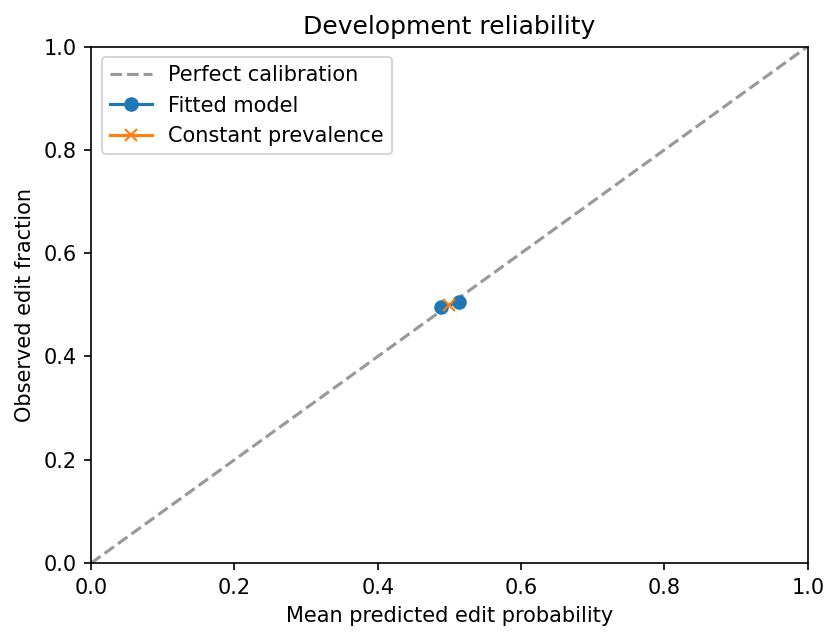
\includegraphics[width=\columnwidth]{figures/receipt-residual-reliability.png}
\caption{Reliability on development for the selected residual checkpoint. Probabilities cluster near the balanced class prevalence.}
\end{figure}

Development ECE was 0.0080 and Brier score was 0.24990 versus 0.25000 for constant prevalence. Historical WildReceipt and XFUND ECE were 0.0106 and 0.0284; constant prevalence had better Brier scores on both. The confidence gate deferred all 400 development receipts. At confidence 0.50, the binary classifier covered all 400 with 49.5\% error. WildReceipt preview coverage was 12/2,672, with six errors among the 12 accepted. Accepted error is undefined at zero coverage.
\section{Optimization under a review budget}
The timing path includes file decode, orientation, tile extraction, model forward, pooling, calibration, decision and serialization. We timed one receipt at a time on a Ryzen 7 5800U with two intra-op threads, eight warm-ups per model, and rotating model order across 400 receipts. INT8 uses actual quantized operators. The PatchNet distilled student learned from the earlier full-RGB teacher and has a matched hard-label control.

\begin{table}[t]
\caption{Measured costs at the same 40-review budget. Each design found 21 edits and raised 19 false flags.}
\centering\footnotesize
\begin{tabular}{lrrr}
\toprule Design & Size (MiB) & Median (ms) & p95 (ms) \\ \midrule
Residual FP32 & 3.653 & 156.46 & 970.29 \\
Residual INT8 & 1.159 & 241.07 & 1,590.80 \\
PatchNet hard & 0.054 & 86.92 & 551.93 \\
PatchNet distilled & 0.054 & 86.28 & 534.57 \\
\bottomrule
\end{tabular}
\end{table}

\begin{figure}[t]
\centering
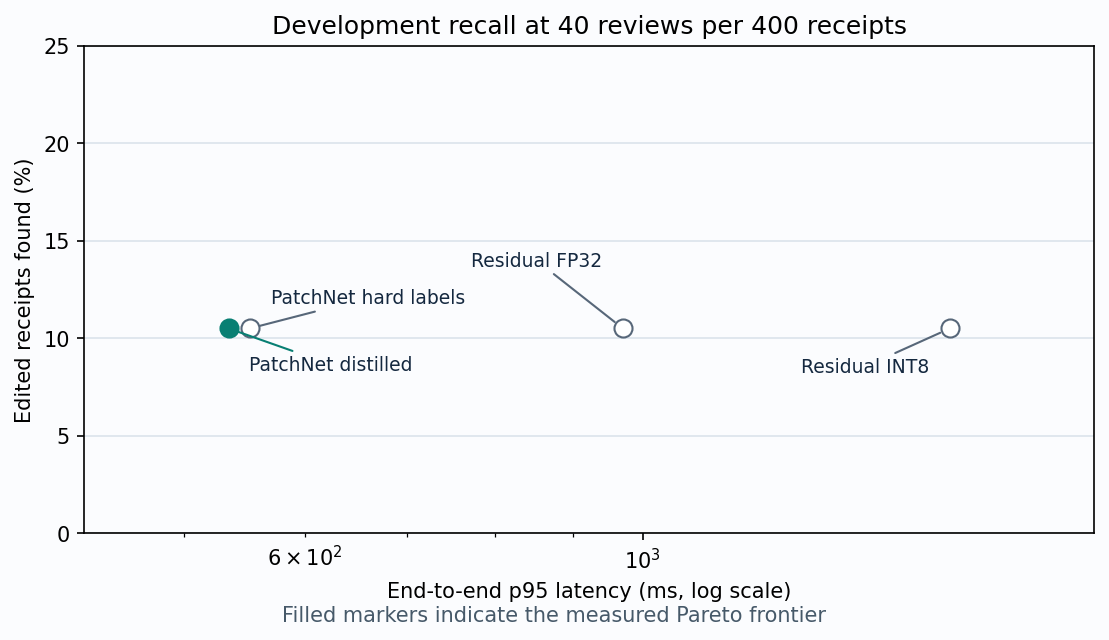
\includegraphics[width=\columnwidth]{figures/receipt-pareto-v1/recall-vs-p95.png}
\caption{Recall versus p95 end-to-end latency. Dominance refers to these measured point estimates.}
\end{figure}

At equal recall, both students dominate both residual variants on size. Distilled PatchNet led the observed p95 frontier; one pass cannot establish a repeatable latency benefit over the hard-label student. Only the students met the median target. Under uniform selection of 40 of the 400 documents, of which 200 are edits, the expected count is 20. The exact central 95\% randomization interval is 14 to 26 edits. Random review finds at least the measured 21 with probability 0.434.
\begin{figure}[t]
\centering
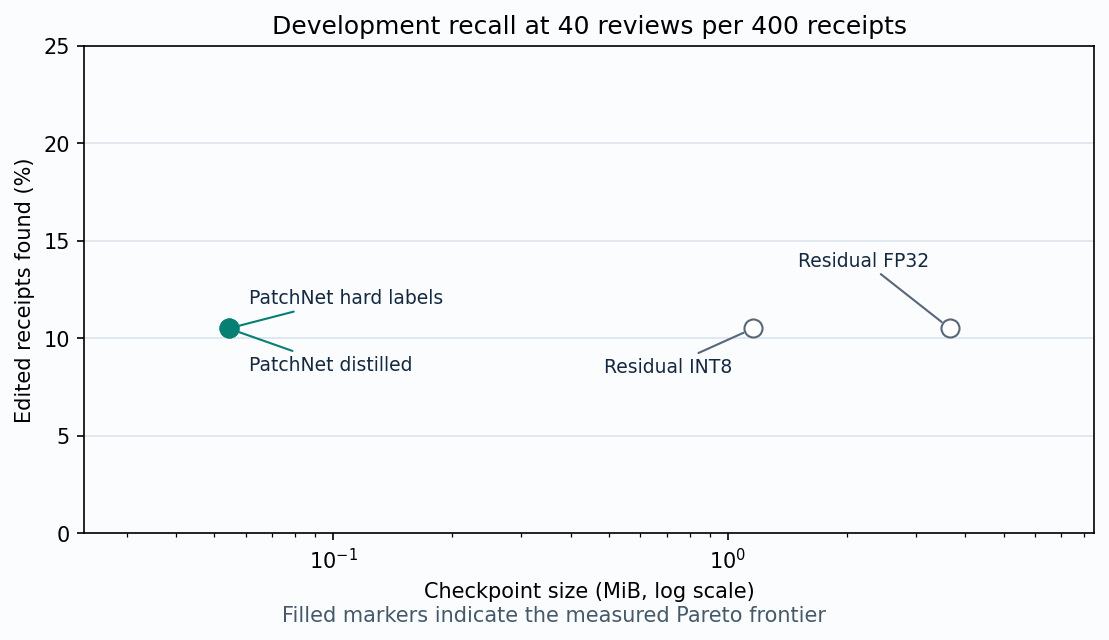
\includegraphics[width=\columnwidth]{figures/receipt-pareto-v1/recall-vs-size.png}
\caption{Recall versus checkpoint size. Both PatchNet students tie on this frontier.}
\end{figure}

Three additional passes on the first 40 hash-ordered development receipts gave FP32 medians of 127--136 ms at two threads and 110--125 ms at four threads. All logits agreed with previous scores within 0.0001. The distilled minus hard-label paired median difference was -1.15 ms (source-bootstrap 95\% interval [-1.63, -0.18]); their p95 ordering changed across passes. The panel supports a small typical difference but leaves the tail ranking uncertain.

\section{Robustness and error mechanisms}
We compared 24 development pairs under clean and perturbed conditions at frozen calibration. Strong blur raised recall and FPR from 8.33\% to 25\%; strong low light reduced both to zero. JPEG quality 42 moved AUROC from 0.5156 to 0.4905, with paired 95\% interval for the change [-0.1025, +0.0178]. Large random and edit-targeted occlusions yielded AUROCs 0.5052 and 0.4991. The latter covered 80.5\% of edited pixels on average. All ten degradation intervals for AUROC included zero. The demo deferred 13/13 open-set uploads and 48/48 clean controls. OOD-specific rejection remains unproven.

Replacing the top tile with gray lowered its score relative to a matched off-mask deletion in 48/48 images. The mean advantage was 0.0845 logits [0.0634, 0.1103]. Gray replacement can introduce new edges. Restricting the pool to edit-intersecting tiles ranked edits higher in 18/24 pairs. Background-only scores tied in 24/24, but falsely flagged two genuine receipts. Full-document pooling ranked edits higher in 7/24 pairs with 14 ties. These interventions distinguish a score-influencing highlight from correct localization.

We extended the pooling probe to all 200 development pairs. Restricting the pool to annotated edit tiles ranked the edit higher in 144 pairs (72\%). Ordinary document pooling did so in 43 (21.5\%) and tied in 137 (68.5\%). Background-only pooling tied in all 200. For masks below 0.5\% of document area, edit-site versus document wins were 80/99 versus 27/99; for larger masks they were 64/101 versus 16/101. The oracle uses annotations and cannot serve as an inference policy.

Case A: deleting a false-flagged genuine tile moved the logit from 1.858 to 1.750, still above the 1.431 cutoff. Mine genuine training receipts with multiple high-scoring tiles and measure FPR at matched recall. Case B: a genuine background alone scored 1.730; the matched edit site scored 1.341. Penalize off-edit tiles and recheck the 2/24 background false flags.

Case C: shifting the grid moved a missed edit from 0.347 to 0.615, yet the strongest tile still missed the mask. Compare overlap against 29/200 development localization hits and measure p95 latency. Case D: the highlighted tile covered 2,294 edited pixels but even top-one pooling gave only 0.337. Test stronger paired supervision and count localized misses. Case E: restoring 1,176 edited pixels reduced the score from 0.368 to 0.289. Test adjacent-tile aggregation for elongated edits and track both genuine FPR and recovered edits.
\begin{figure}[t]
\centering
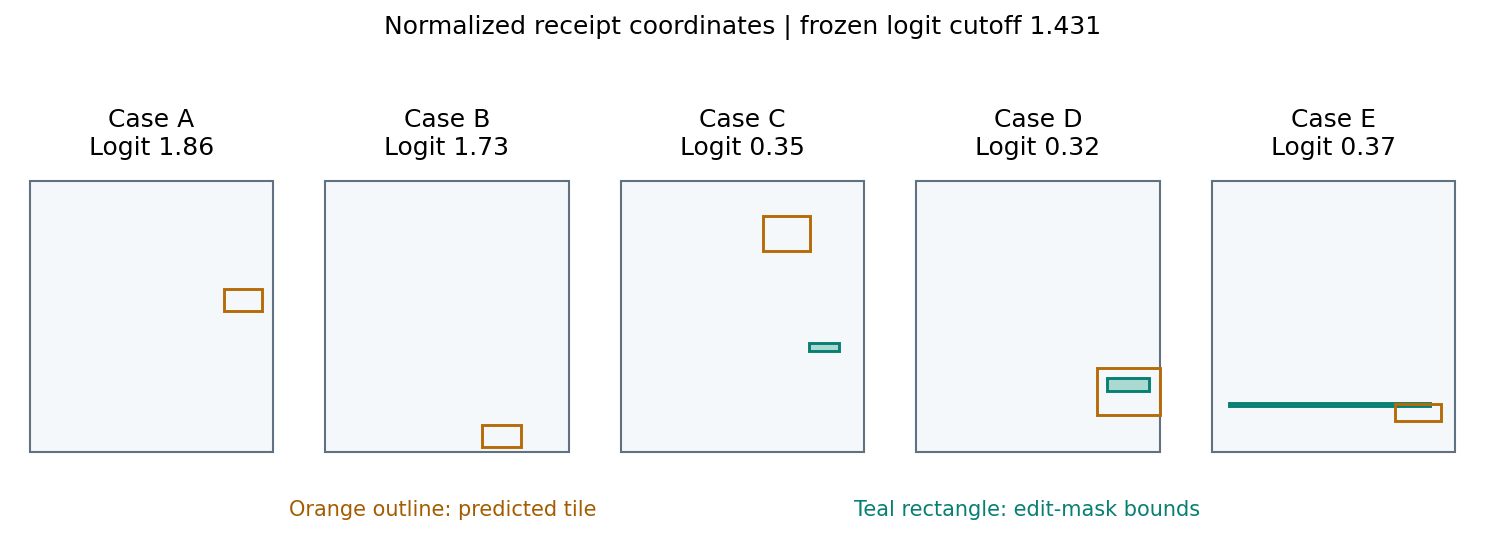
\includegraphics[width=\columnwidth]{figures/receipt-explain-v1/case-geometry.png}
\caption{Five development cases. Each schematic shows the selected tile and the annotated edit bounds, where present. A tile can influence a false flag or intersect a real edit that the model still misses.}
\end{figure}

\section{Reproduction and limitations}
The project records pinned dependencies, per-seed configurations, source-group manifests, fitted checkpoint hashes, calibration parameters, and local per-document scores. The selected three-epoch fit took 26.6 seconds on CPU excluding input preparation. The Streamlit app verifies its local checkpoint and calibration digests and returns an edit estimate, confidence, evidence tile, queue outcome, and advice. Uploaded images are processed locally. The historical two-document Studio uses registered SSIM and addresses reference comparison.

TorchVision publishes the source and revision of the pretrained weights [3]. Its software license is BSD-3-Clause. Its documentation distinguishes software and pretrained-weight terms. Explicit terms for this exact checkpoint remain unresolved in the study record. The reproduction guide identifies the official download and SHA-256. The exploratory TruFor [4] panel has limited scope; incomplete full-cohort scoring supplies no full-cohort estimate.

A fresh confirmatory test requires newly authorized receipt sources. Both detectors must be calibrated on separate sources and locked with the same eligibility rules and evaluation manifests before either scores the new cohorts. Historical WildReceipt and held-back XFUND answer narrower questions. The evidence supports standard manual review for actual reimbursement claims.
\section*{Contributions}
Mohsin Saeed (2024307) coordinated the project, proposed the idea, and chose the architecture. Hamza Sami (2024212) ran the experiments and recorded the results. M. Taha (2024475) prepared the documentation and performed quality assurance.
\begin{thebibliography}{4}
\bibitem{data} Scam AI, AIForge-Doc-v2, dataset card and paired-image release. \url{https://huggingface.co/datasets/Scam-AI/AIForge-Doc-v2}
\bibitem{mobile} A. Howard et al., Searching for MobileNetV3, Proc. IEEE/CVF International Conference on Computer Vision, 2019.
\bibitem{vision} TorchVision, MobileNetV3 Small, ImageNet-1K V1 initialization and pretrained-model documentation. \url{https://docs.pytorch.org/vision/stable/models.html}
\bibitem{trufor} F. Guillaro et al., TruFor: Leveraging All-Round Clues for Trustworthy Image Forgery Detection and Localization, Proc. IEEE/CVF Conference on Computer Vision and Pattern Recognition, 2023.
\end{thebibliography}
\end{document}
